\subsection{Búsquedas geolocalizadas}


\begin{frame}[t]\frametitle{Búsquedas geolocalizadas}

La búsqueda geolocalizada es una herramienta que nos da la posibilidad de obtener tuits generados en un área geográfica particular. Para esto, primero intenta buscar tuits cuyas coordenadas sean las buscadas.


\begin{columns}
    \begin{column}{0.30\textwidth}
        \begin{figure}
            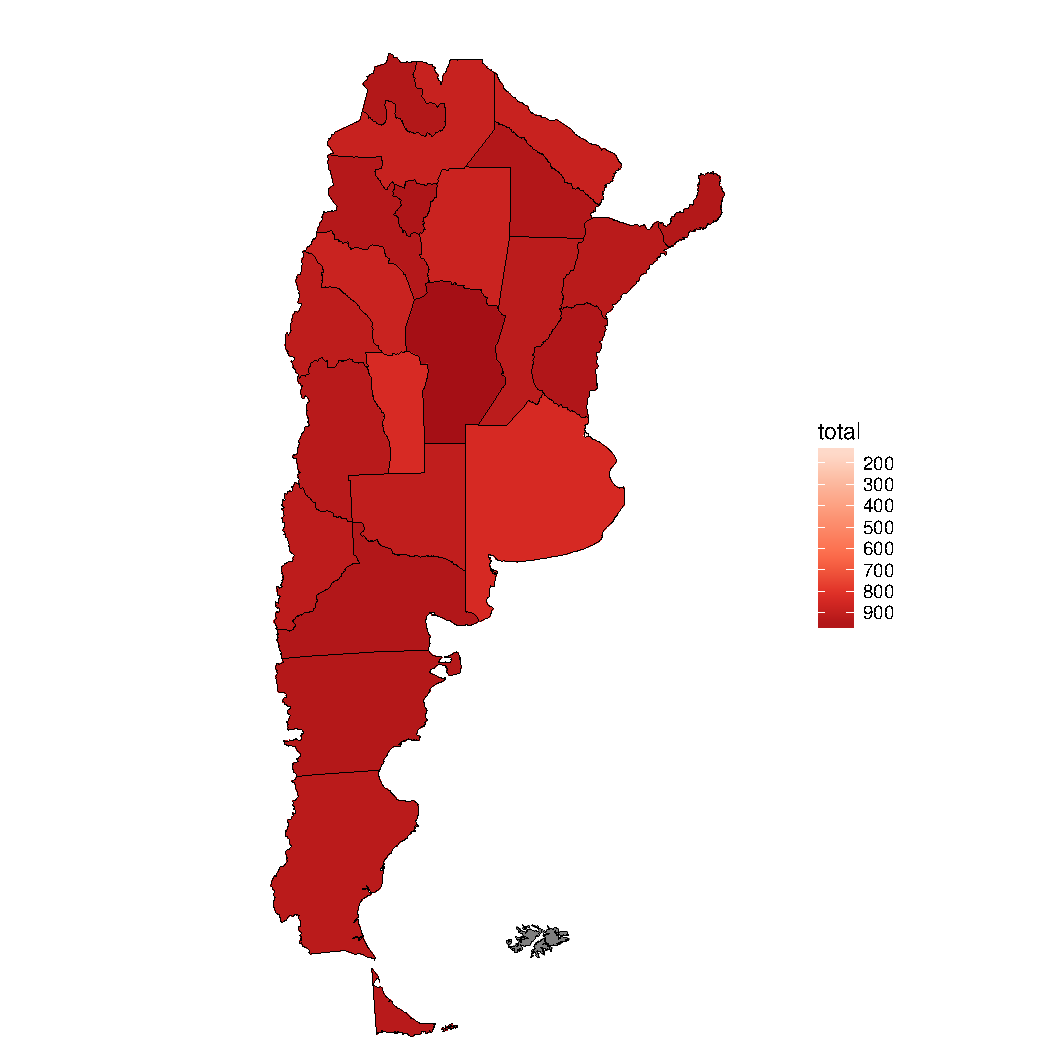
\includegraphics[width=\linewidth]{../src/images/mapaprovincias.pdf}
            % \caption{} 
            \label{fig:mapaProvincias}
        \end{figure}
    \end{column}

    \begin{column}{0.30\textwidth}
        \begin{figure}
            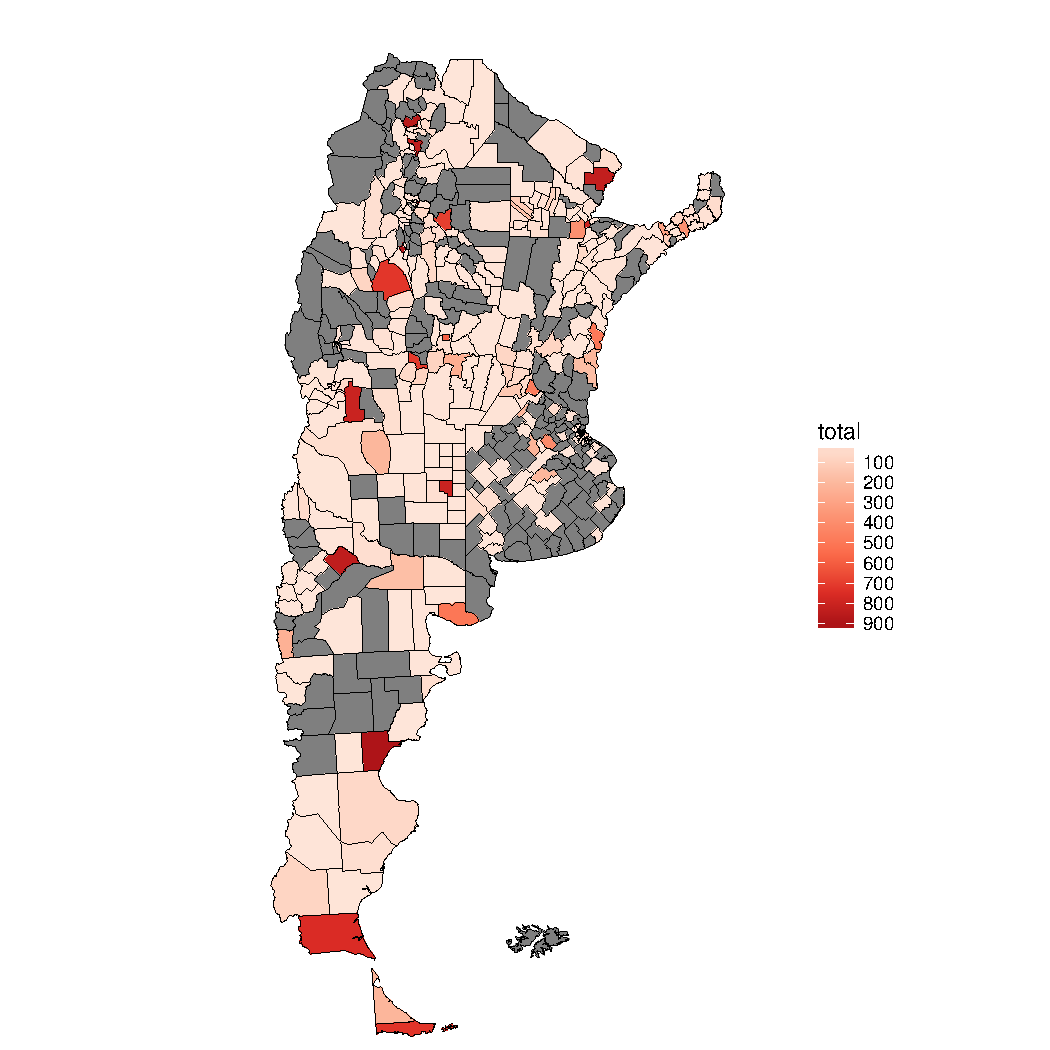
\includegraphics[width=\linewidth]{../src/images/mapadepartamentos.pdf}
            % \caption{} 
            \label{fig:mapaDepartamentos}
        \end{figure}
    \end{column}

    \begin{column}{0.30\textwidth}
        \begin{figure}
            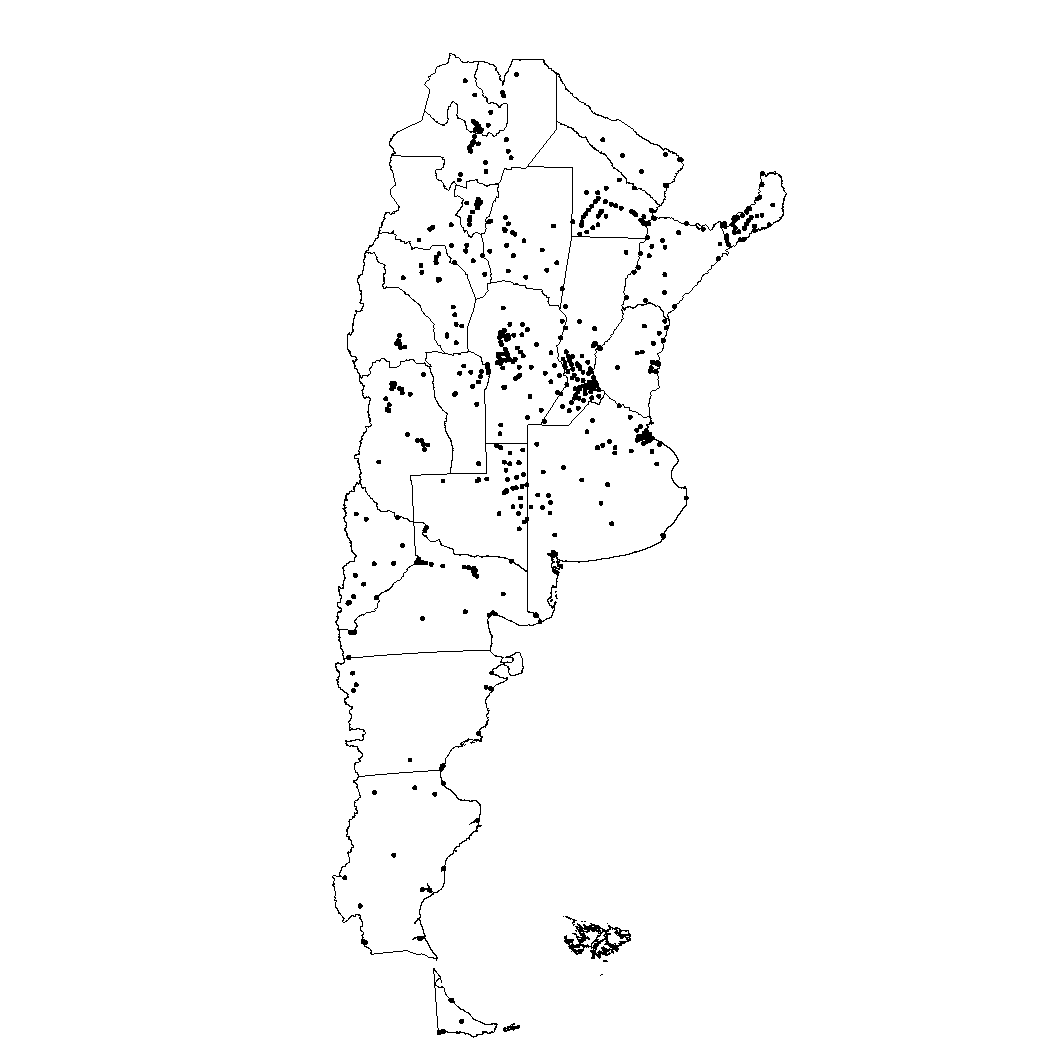
\includegraphics[width=\linewidth]{../src/images/mapaprovinciasConPuntos.pdf}
            % \caption{} 
            \label{fig:mapaPuntos}
        \end{figure}
    \end{column}
\end{columns}

Se realizaron búsquedas por cada provincia con centro en las coordenadas de los departamentos de la misma y con un radio de 20 millas. 

Nos quedamos con los usuarios que tienen como campo \textit{location} al menos uno de los nombres de las ciudades de la provincia. 



\end{frame}

\subsection{Tokenización y normalización}

\begin{frame}[t]\frametitle{Tokenización y normalización del texto}
    \begin{block}{Tokenización}
    Se consideró una palabra a las secuencias de caracteres formados únicamente por letras. Por lo tanto se eliminaron las menciones con @, los hashtags y links entre otros. Decidimos ignorar estos términos ya que no tienen interés lingüístico y agregarían mucho ruido a los datos.
    \end{block}

    \begin{block}{Normalización}
    Todas las letras se convirtieron a letra minúscula y las palabras con más de tres letras iguales de forma consecutiva se redujeron para que solo tengan tres repeticiones. De esta forma, el término \textit{padreeeee} y \textit{padreeee} fueron reducidos a una única unidad léxica (\textit{padreee}). Esto se hizo con la librería \textit{TweetTokenizer de NLTK}. 
    \end{block}

\end{frame}
